\documentclass[12pt]{article}
\usepackage[utf8]{inputenc}
\usepackage{xcolor}
\usepackage{graphicx} % Allows you to insert figures
\usepackage{amsmath} % Allows you to do equations
\usepackage{fancyhdr} % Formats the header\
\usepackage{geometry} % Formats the paper size, orientation, and margins
\usepackage[style=authoryear-ibid,backend=biber]{biblatex} % Allows you to do citations - does Harvard style and compatible with Zotero
\addbibresource{Example.bib} % Tells LaTeX where the citations are coming from. This is imported from Zotero
\usepackage[english]{babel}
\usepackage{csquotes}
\renewcommand*{\nameyeardelim}{\addcomma\space} % Adds comma in in-text citations
\linespread{1.25} % About 1.5 spacing in Word
\setlength{\parindent}{0pt} % No paragraph indents
\setlength{\parskip}{1em} % Paragraphs separated by one line
\renewcommand{\headrulewidth}{0pt} % Removes line in header
\geometry{legalpaper, portrait, margin=1in}
\setlength{\headheight}{14.49998pt}

\begin{document}
\begin{titlepage}
   \begin{center}
        \vspace*{0.25cm}

        \Huge\underline{\textbf{CYCLONE ARCADE}}
        \Huge\underline{\textbf{LED CHASER GAME}}

        \vspace{0.5cm}
        % \LARGE{optional subtitle below}
            
        \vspace{3 cm}
        % \Large{Group Name}
       
        \vspace{0.25cm}
        \large{By-                    
        
        DIVYANSH TANWAR (2020UEC2572) 

MUKUL GUPTA (2020UEC2612) 

YASH GUPTA (2020UEC2619) }
       
        \vspace{3 cm}
        % \Large{Month Day, Year}https://www.overleaf.com/project/61f783ee19dc0d4cef25dcfb
        
        \vspace{0.25 cm}
        \Large{ECECC09 Electronic Design Workshop LAB PROJECT 

ECE Division 

Netaji Subhas University of Technology 

Sector-3, Dwarka, New Delhi 110078 }
       

       \vfill
    \end{center}
\end{titlepage}

\setcounter{page}{2}
\pagestyle{fancy}
\fancyhf{}
\rhead{\thepage}


\section*{\underline{SYNOPSIS}}

This project basically uses a WS2812B LED strip. 

There is a start/stop button which we will use to start the game.

This game contains various levels. 

In a particular level x number of consecutive LED’S are in ‘ON’ state and one circularly rotating Led will be present. If we managed to stop the revolving LED when it is pointing at the ON LED’S, we will win the particular round. There are x number of round and if we are able to win all the round then you are an absolute winner. The subsequent round will become more tougher as compared to previous rounds as the value of x will decrease. 

\section*{\underline{MOTIVATION}}
Is there any person in the world who don’t like game? Definitely not! So, we have designed a very interesting arcade game called as Cyclone Arcade LED Chaser game.

This game can help you relax if you are tired because of long online classes and just want to relax your mind. You all will definitely enjoy this wonderful game and this game will definitely test your hand eye coordination and your reflexes. Kudos to you if you win!

\section*{\underline{PROJECT DESCRIPTION}}
The various components that will be used in our project are as follows:
\subsection*{1. ARDUINO (MICROCONTROLLER)}

\begin{flushleft}
Arduino is a prototype platform (open-source) based on easy-to-use hardware and software. It consists of a circuit board, which can be programmed (referred to as a micro-controller) and a ready-made software called Arduino IDE (Integrated Development Environment), which is used to write and upload the computer code to the physical board.  
\end{flushleft}
\centering
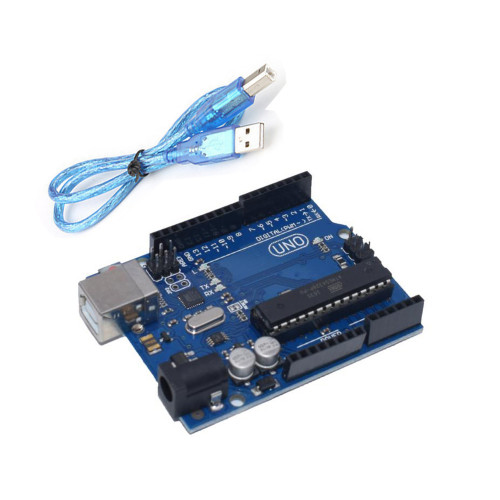
\includegraphics[width=7cm]{arduino.jpg}


\begin{flushleft}
\subsection*{2. PUSH BUTTON}
\end{flushleft}

\begin{flushleft}
Push button will be used to play the game. The player will push the button to position the moving light in the correct place and orientation.
\end{flushleft}

\centering
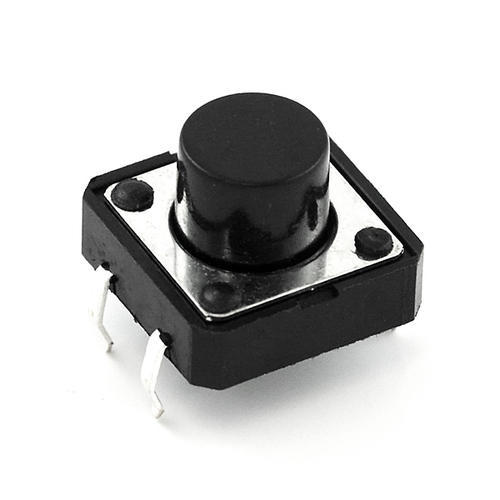
\includegraphics[width=5cm]{pushbutton.jpg}


\begin{flushleft}
\subsection*{3. WS2812b LED Strip}
\end{flushleft}
\begin{flushleft}
WS2812B is an intelligent control LED light source that the control circuit and RGB chip are integrated in a package of 5050 components. These flexible RGB LED strips are an easy way to add complex lighting effects to a project. Each LED has an integrated driver that allows you to control the colour and brightness of each LED independently.
\end{flushleft}

\centering
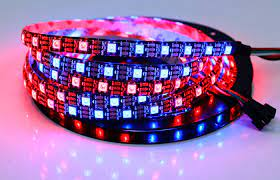
\includegraphics[width=8cm]{led.jpg}


\pagebreak

\section*{\underline{BLOCK DIAGRAM}}
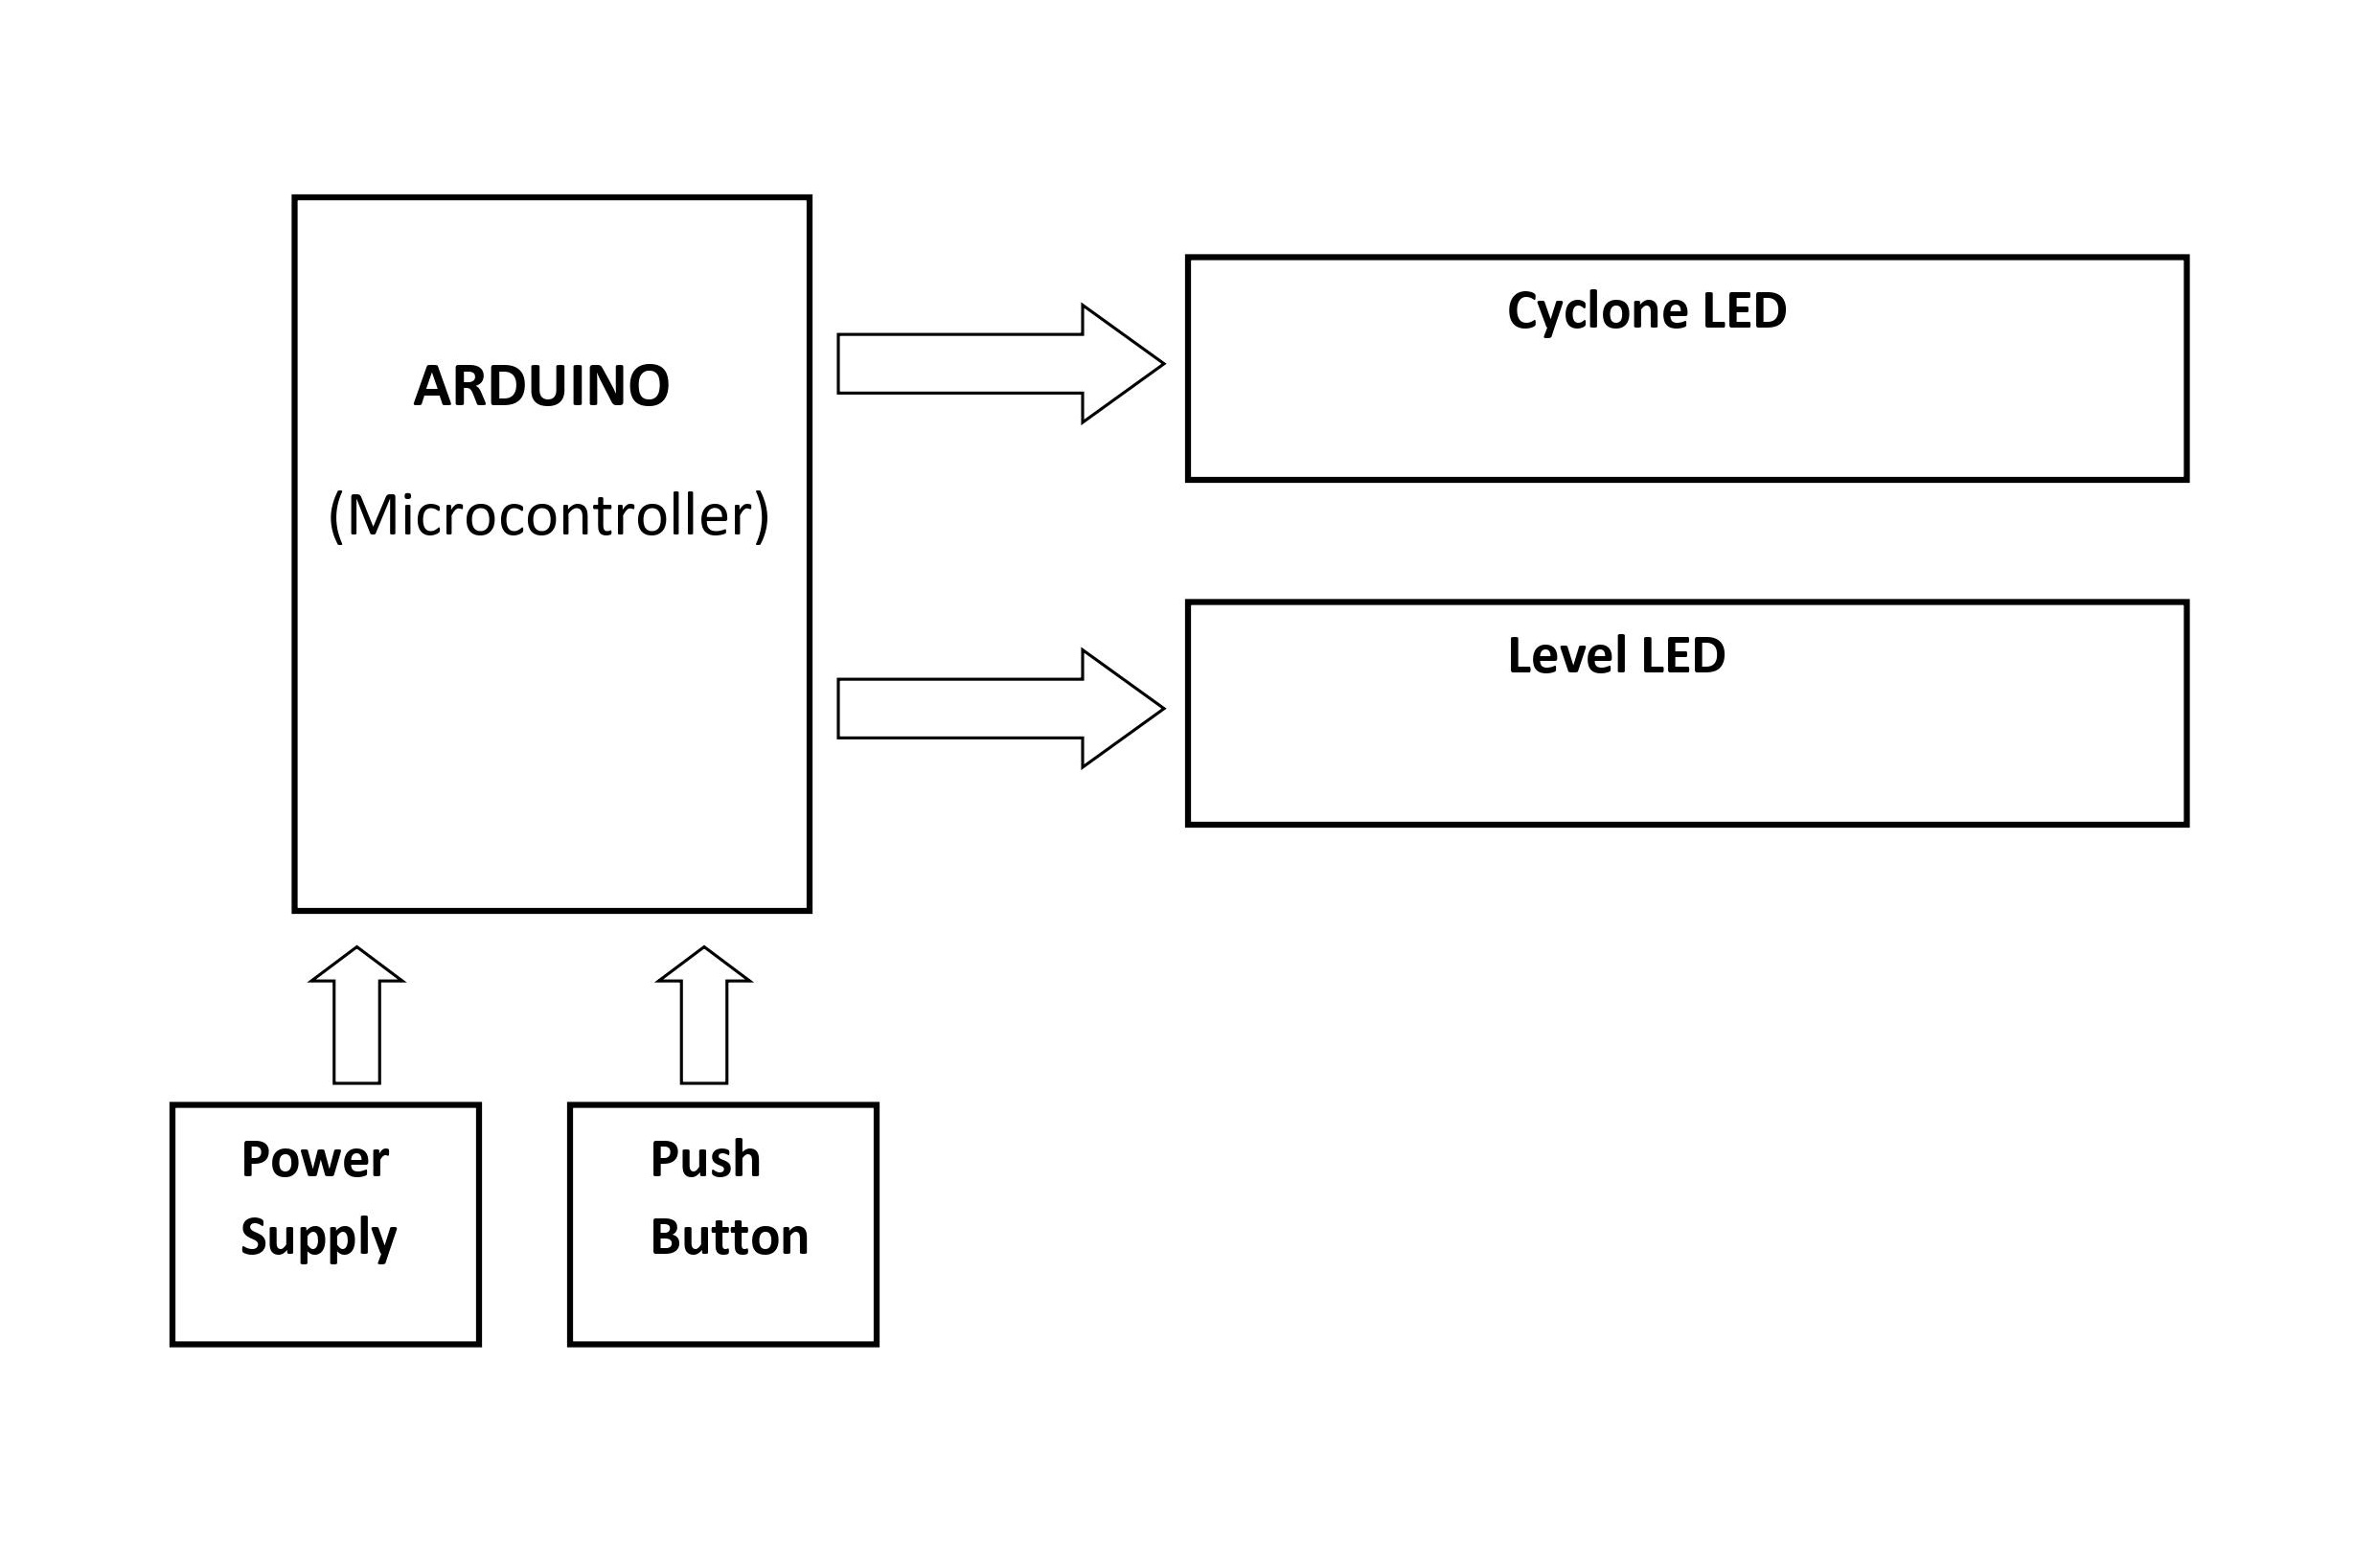
\includegraphics[width=15cm]{block.jpg}
\section*{\underline{FLOW CHART}}
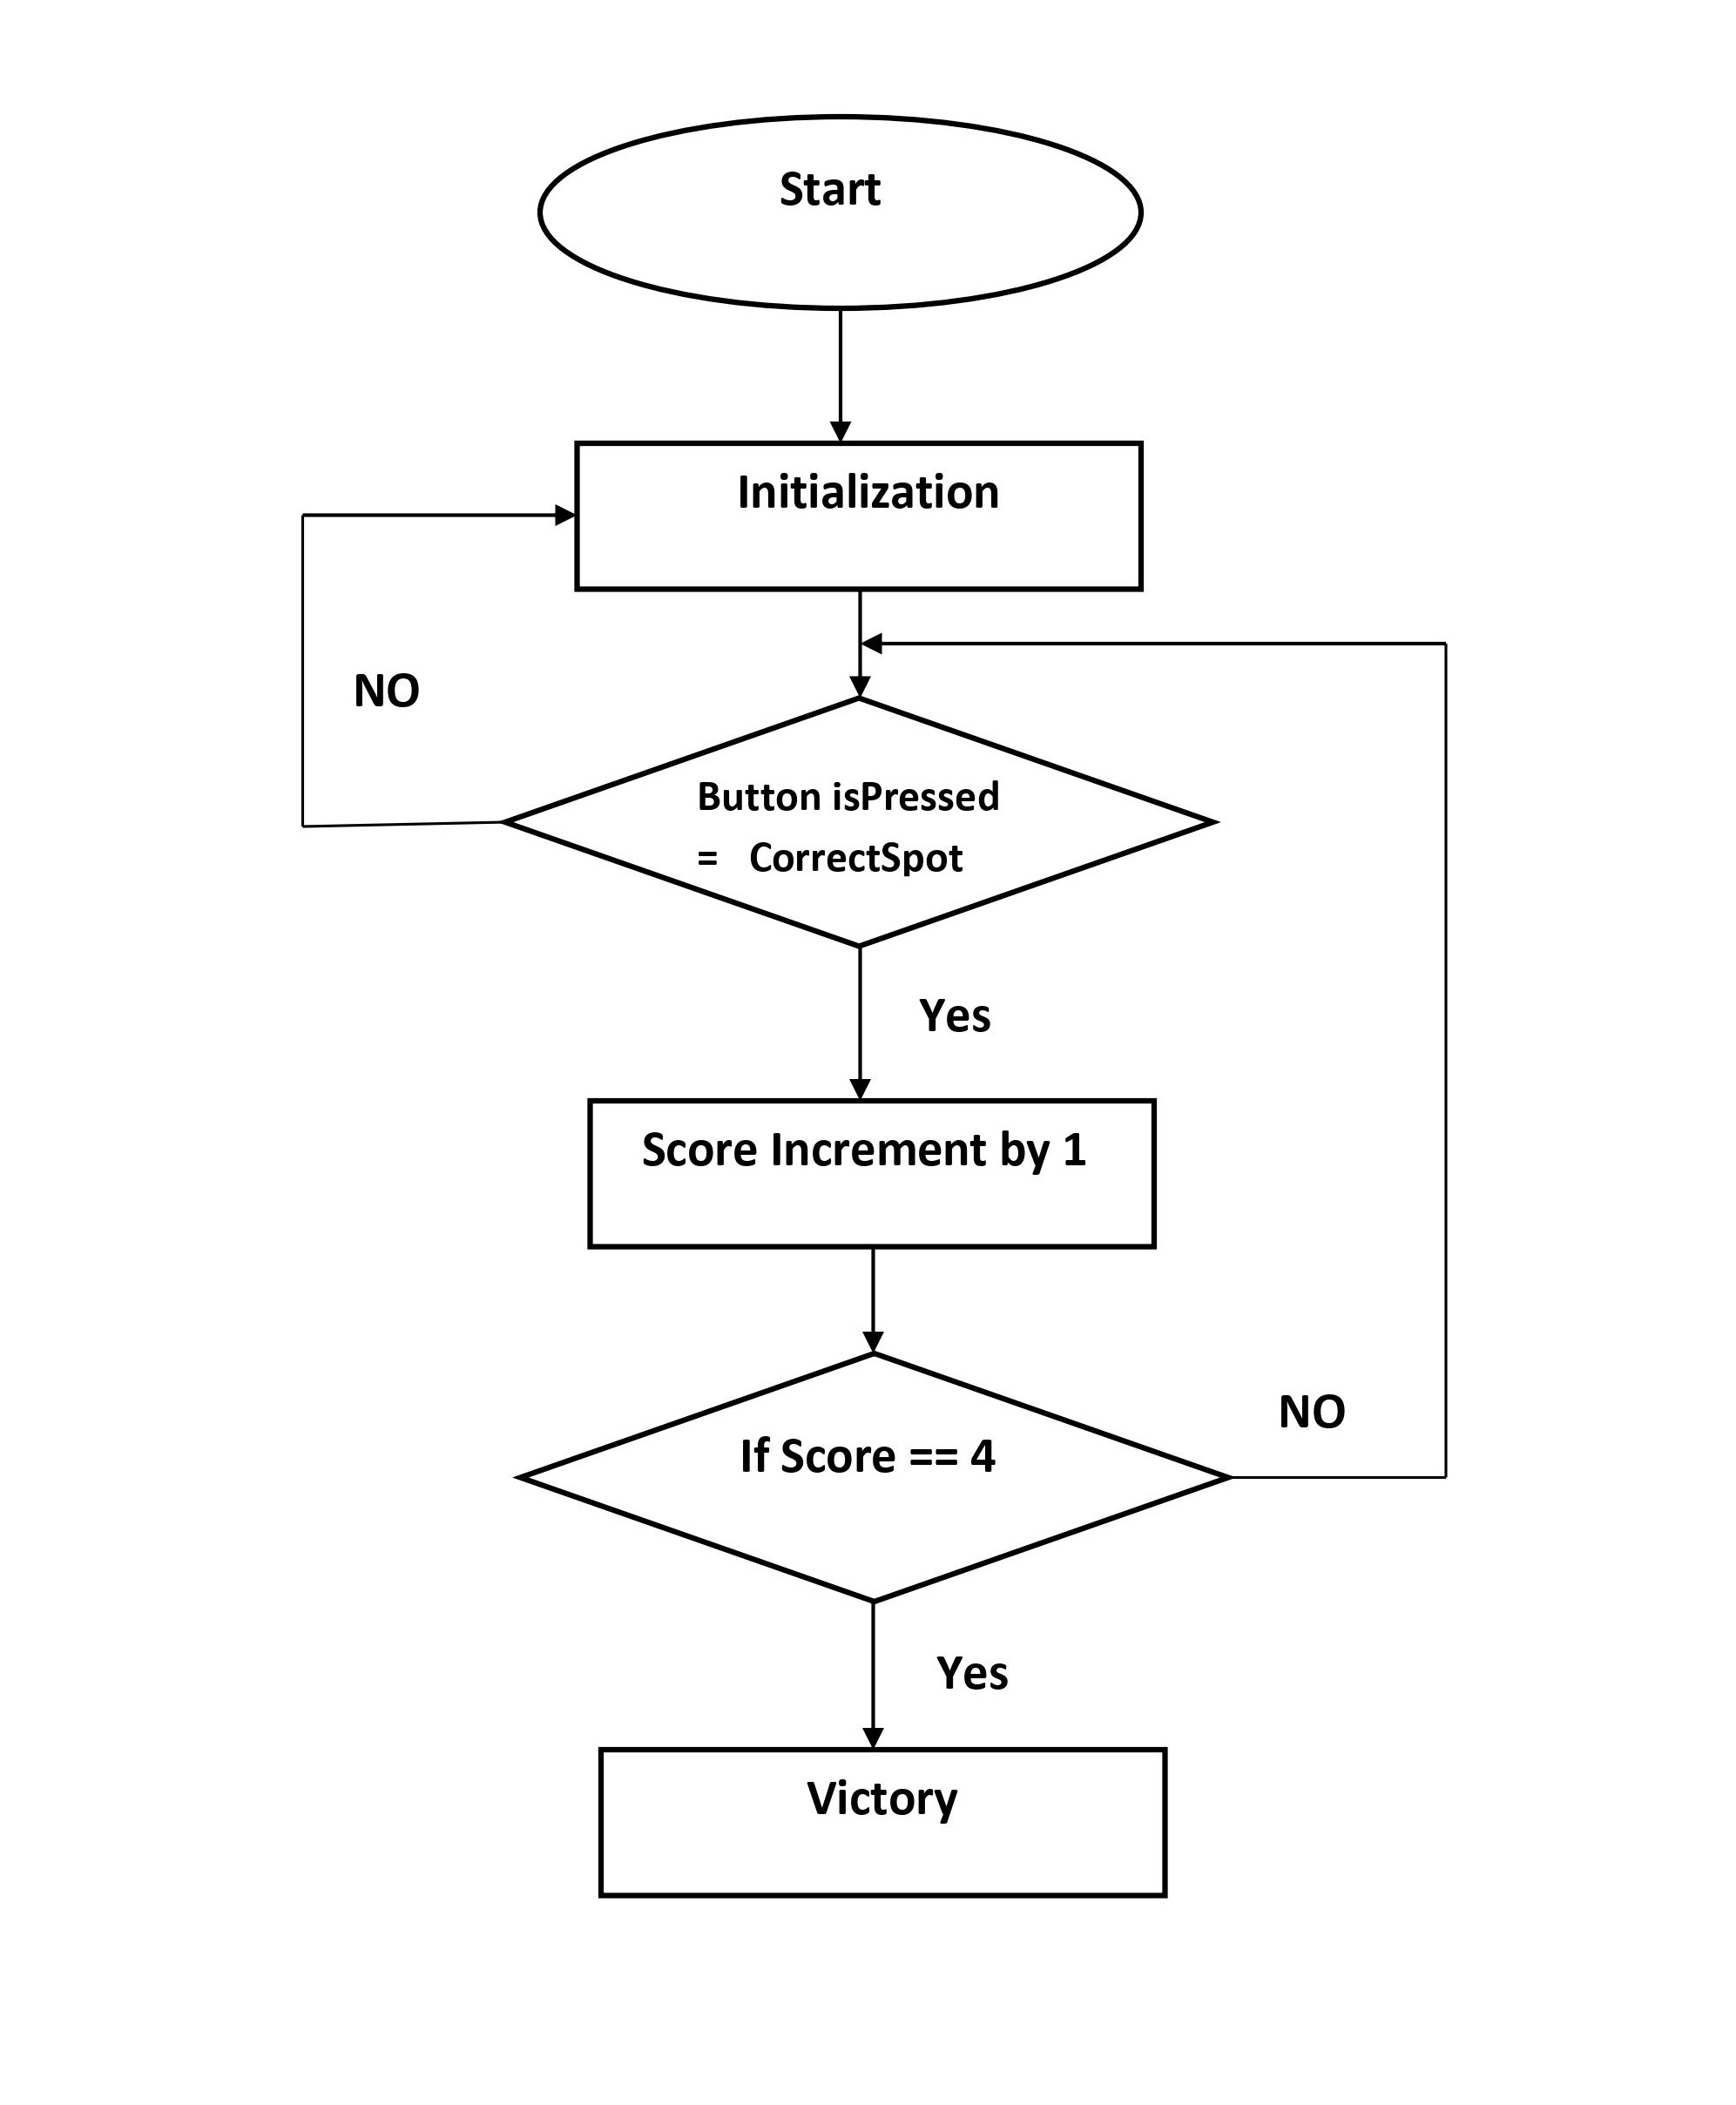
\includegraphics[width=13cm]{flow.jpg}

\pagebreak
\section*{\underline{BILL OF MATERIALS}}
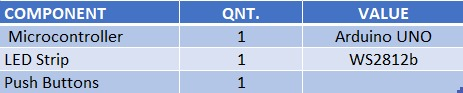
\includegraphics[width=15cm]{bill.jpg}


\section*{\underline{GANTT CHART}}
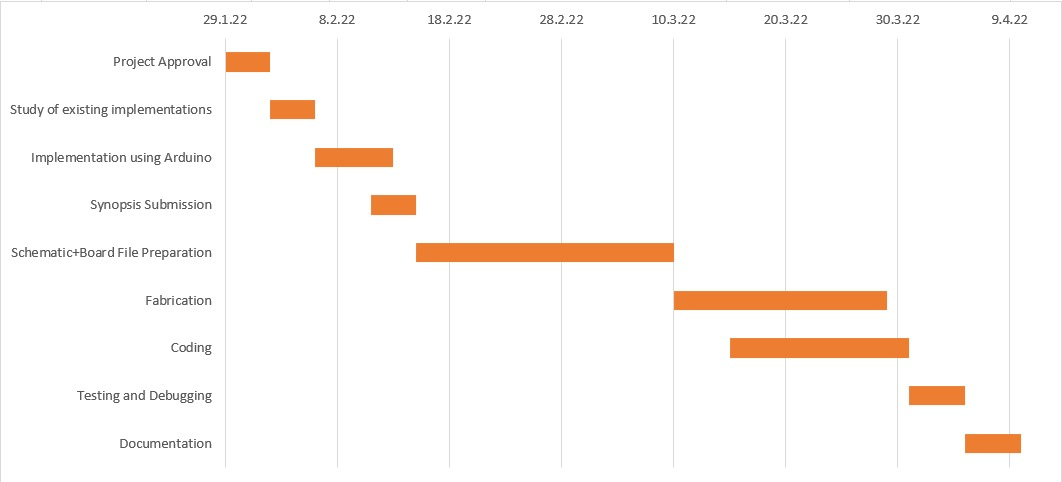
\includegraphics[width=18cm]{gantt.jpeg}

\end{document}
